Considere el ``globo de la muerte'' que se ilustra en la figura de este problema. Sea $R$ = 2.0 m su radio, $m$ = 150 kg la masa del conjunto de motocicleta y motociclista, y $v$ = 6.0 m/s la velocidad de la máquina al pasar por el punto $A$ (tome $g$ = 10 m/s2). En este punto:
\begin{enumerate}
    \item ¿Cuál es el valor de la fuerza centrípeta que actúa sobre el conjunto de máquina y conductor?
    \item ¿Cual es el valor de la reacción normal del globo sobre el conjunto?
\end{enumerate}
\begin{figure}[htb]
  \centering
  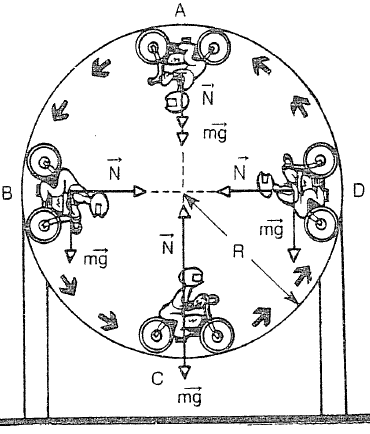
\includegraphics[scale=0.55]{figuras/fig_alvarenga_p222_32.png}
  \caption{Problema 5}
\end{figure}
